% THIS DOCUMENT IS FOLLOWS THE VOLERE TEMPLATE BY Suzanne Robertson and James Robertson
% ONLY THE SECTION HEADINGS ARE PROVIDED
%
% Initial draft from https://github.com/Dieblich/volere
%
% Risks are removed because they are covered by the Hazard Analysis
\documentclass[12pt]{article}
\usepackage{graphicx}
\usepackage{float}

\usepackage{booktabs}
\usepackage{tabularx}
\usepackage{hyperref}
\hypersetup{
    bookmarks=true,         % show bookmarks bar?
      colorlinks=true,      % false: boxed links; true: colored links
    linkcolor=red,          % color of internal links (change box color with linkbordercolor)
    citecolor=green,        % color of links to bibliography
    filecolor=magenta,      % color of file links
    urlcolor=cyan           % color of external links
}

\newcommand{\lips}{\textit{Insert your content here.}}

%% Comments

\usepackage{color}

\newif\ifcomments\commentstrue %displays comments
%\newif\ifcomments\commentsfalse %so that comments do not display

\ifcomments
\newcommand{\authornote}[3]{\textcolor{#1}{[#3 ---#2]}}
\newcommand{\todo}[1]{\textcolor{red}{[TODO: #1]}}
\else
\newcommand{\authornote}[3]{}
\newcommand{\todo}[1]{}
\fi

\newcommand{\wss}[1]{\authornote{blue}{SS}{#1}} 
\newcommand{\plt}[1]{\authornote{magenta}{TPLT}{#1}} %For explanation of the template
\newcommand{\an}[1]{\authornote{cyan}{Author}{#1}}

%% Common Parts

\newcommand{\progname}{Scanalyze AI} % PUT YOUR PROGRAM NAME HERE
\newcommand{\authname}{Team 16, Ace
\\ Hamza Issa
\\ Ahmad Hamadi
\\ Jared Paul
\\ Gurnoor Bal} % AUTHOR NAMES                  

\usepackage{hyperref}
    \hypersetup{colorlinks=true, linkcolor=blue, citecolor=blue, filecolor=blue,
                urlcolor=blue, unicode=false}
    \urlstyle{same}
                                


\begin{document}

\title{Software Requirements Specification for \progname: subtitle describing software} 
\author{\authname}
\date{\today}
	
\maketitle

~\newpage

\pagenumbering{roman}

\tableofcontents

~\newpage

\section*{Revision History}

\begin{tabularx}{\textwidth}{p{3cm}p{2cm}X}
\toprule {\textbf{Date}} & {\textbf{Version}} & {\textbf{Notes}}\\
\midrule
Date 1 & 1.0 & Notes\\
Date 2 & 1.1 & Notes\\
\bottomrule
\end{tabularx}

~\\

~\newpage
\section{Purpose of the Project}
\subsection{User Business}
\lips
\subsection{Goals of the Project}
\lips
\section{Stakeholders}
\subsection{Client}
\lips
\subsection{Customer}
\lips
\subsection{Other Stakeholders}
\lips
\subsection{Hands-On Users of the Project}
\lips
\subsection{Personas}
\lips
\subsection{Priorities Assigned to Users}
\lips
\subsection{User Participation}
\lips
\subsection{Maintenance Users and Service Technicians}
\lips

\section{Mandated Constraints}
\subsection{Solution Constraints}
\lips
\subsection{Implementation Environment of the Current System}
\lips
\subsection{Partner or Collaborative Applications}
\lips
\subsection{Off-the-Shelf Software}
\lips
\subsection{Anticipated Workplace Environment}
\lips
\subsection{Schedule Constraints}
\lips
\subsection{Budget Constraints}
\lips
\subsection{Enterprise Constraints}
\lips

\section{Naming Conventions and Terminology}
\subsection{Glossary of All Terms, Including Acronyms, Used by Stakeholders
involved in the Project}
\lips

\section{Relevant Facts And Assumptions}
\subsection{Relevant Facts}
\lips
\subsection{Business Rules}
\lips
\subsection{Assumptions}
\lips

\section{The Scope of the Work}
\subsection{The Current Situation}
\lips
\subsection{The Context of the Work}
\lips
\subsection{Work Partitioning}
\lips
\subsection{Specifying a Business Use Case (BUC)}
\lips

\section{Business Data Model and Data Dictionary}
\subsection{Business Data Model}
\begin{figure}[H]
    \centering
    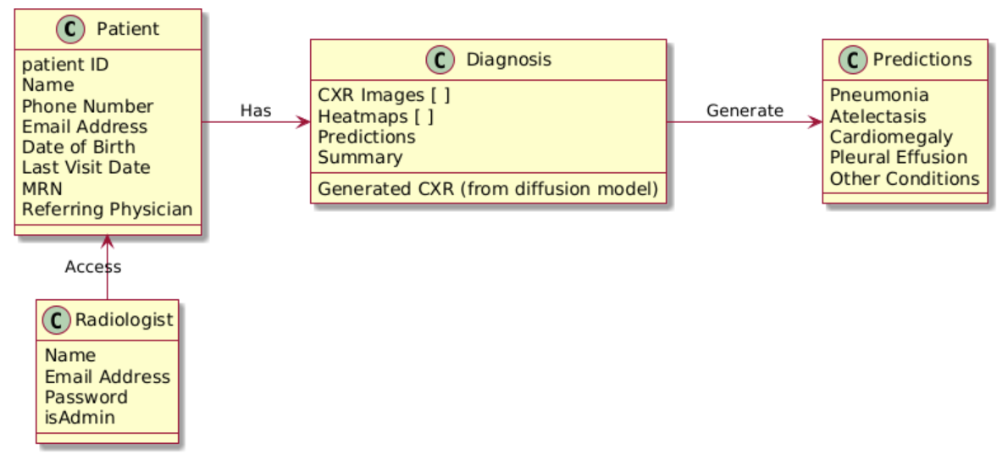
\includegraphics[width=0.8\textwidth]{images/bussiness_data_model.png}
    \caption{Business Data Model}
    \label{fig:business_data_model}
\end{figure}
\subsection{Data Dictionary}
\begin{itemize}
    \item \textbf{Patient}: contains all the relevant personal details of the patient, accessed via the database of patients.

    \item \textbf{Radiologist}: contains authentication details and access level for the users that can access the system.

    \item \textbf{Diagnosis}: Diagnostic data from chest X-ray analysis.
    \begin{itemize}
        \item \textbf{CXR Images}: Uploaded chest X-rays.
        \item \textbf{Heatmaps}: Attention maps from X-rays.
        \item \textbf{Predictions}: Probability scores for various conditions.
        \item \textbf{Summary}: Brief diagnostic overview.
        \item \textbf{Generated CXR}: Simulated X-rays from diffusion models.
    \end{itemize}

    \item \textbf{Predictions}: contains all prediction/risk values for the diseases considered.
\end{itemize}


\section{The Scope of the Product}
\subsection{Product Boundary}
The system covers the Automated Chest X-ray Diagnosis lifecycle, from image input to diagnostic report generation using diffusion models. It focuses on detecting lung-related conditions like pneumonia and pleural effusion. Key components include image analysis, disease prediction through diffusion models, a web interface for radiologists, and security for patient data. The application excludes real-time consultations and other imaging types.

\subsection{Product Use Case Table}
The following table summarizes the product use cases for the project's proposed solution:

\begin{table}[h!]
    \centering
    \caption{Product Use Case Table}
    \begin{tabular}{|c|p{12cm}|}
        \hline
        \textbf{Use Case ID} & \textbf{Use Case Summary} \\
        \hline
        PUC1 & Process chest X-ray image using diffusion model \\
        \hline
        PUC2 & Generate disease predictions from processed X-ray \\
        \hline
        PUC3 & Convert predictions into a structured diagnostic report \\
        \hline
        PUC4 & Display the diagnostic findings on the web interface \\
        \hline
        PUC5 & Generate synthetic CXR images for disease analysis \\
        \hline
    \end{tabular}
\end{table}
\subsection{Individual Product Use Cases (PUC's)}
The following are the individual product use cases (PUCs), with a description, lists of actors, preconditions, and postconditions provided for each.

\begin{itemize}
    \item 
    \begin{description}
        \item[Description:] The system takes a chest X-ray image as input and processes it using diffusion models to identify abnormalities.
        \item[Actors:] Diffusion model, chest X-ray image.
        \item[Precondition(s):] Valid chest X-ray image input is provided.
        \item[Postcondition(s):] Processed image with identified abnormalities is generated.
    \end{description}
    
    \item 
    \begin{description}
        \item[Description:] The system generates a comprehensive list of disease predictions based on the processed chest X-ray image.
        \item[Actors:] Diffusion model, disease prediction module.
        \item[Precondition(s):] Processed image with identified abnormalities is provided.
        \item[Postcondition(s):] A list of disease predictions is generated.
    \end{description}
    
    \item 
    \begin{description}
        \item[Description:] The system converts the list of disease predictions into a structured diagnostic report for healthcare professionals.
        \item[Actors:] Prediction list, report generation module.
        \item[Precondition(s):] A list of disease predictions is provided.
        \item[Postcondition(s):] A diagnostic report is generated.
    \end{description}
    
    \item 
    \begin{description}
        \item[Description:] The user interface module displays the diagnostic report for the radiologist or physician.
        \item[Actors:] User interface module, radiologist/physician.
        \item[Precondition(s):] Diagnostic report is provided.
        \item[Postcondition(s):] Diagnostic report is displayed on the web interface.
    \end{description}
    
    \item 
    \begin{description}
        \item[Description:] The system generates synthetic CXR images with specific disease signatures for analysis and training purposes.
        \item[Actors:] Diffusion model, chest X-ray image.
        \item[Precondition(s):] Valid chest X-ray image input is provided.
        \item[Postcondition(s):] Synthetic CXR images with disease signatures are generated.
    \end{description}
\end{itemize}





\section{Functional Requirements}
\subsection{Functional Requirements}

\begin{itemize}
    \item \textbf{FR1: The system shall accept and read CXR (Chest X-ray) images as input.}
    \begin{itemize}
        \item \textbf{Rationale:} This is the primary input to the diffusion model for disease signature generation.
        \item \textbf{Fit Criterion:} The system can successfully process CXR images and recognize valid formats.
        \item \textbf{Product Use Case(s):} PUC1
    \end{itemize}
    
    \item \textbf{FR2: The system shall process CXR images using a diffusion model to generate disease signatures at specified locations.}
    \begin{itemize}
        \item \textbf{Rationale:} This model allows the system to modify the original image by adding disease-specific patterns for diagnosis.
        \item \textbf{Fit Criterion:} The system generates an output image with added disease signatures based on user-defined specifications.
        \item \textbf{Product Use Case(s):} PUC1, PUC2
    \end{itemize}
    
    \item \textbf{FR3: The system shall identify and classify multiple diseases in the CXR image, including (but not limited to) Pneumonia, Atelectasis, Cardiomegaly, and Pleural Effusion.}
    \begin{itemize}
        \item \textbf{Rationale:} The goal is to detect and classify common lung and cardiac conditions.
        \item \textbf{Fit Criterion:} The system detects the presence or absence of diseases with an accuracy greater than 90\% for each disease.
        \item \textbf{Product Use Case(s):} PUC2, PUC5
    \end{itemize}
    
    \item \textbf{FR4: The system shall generate a structured diagnostic report from the findings on the CXR image.}
    \begin{itemize}
        \item \textbf{Rationale:} Medical professionals need a clear report outlining the findings and severity of the conditions detected.
        \item \textbf{Fit Criterion:} The system generates a report detailing the diseases, their severity, and the locations in the image where the abnormalities were detected.
        \item \textbf{Product Use Case(s):} PUC3, PUC4
    \end{itemize}
    
    \item \textbf{FR5: The system shall display heatmaps on the CXR images to indicate the locations of the detected disease signatures.}
    \begin{itemize}
        \item \textbf{Rationale:} The heatmaps assist radiologists in pinpointing the areas of concern for further analysis.
        \item \textbf{Fit Criterion:} The system overlays heatmaps on the CXR images and accurately highlights regions where disease signatures are present.
        \item \textbf{Product Use Case(s):} PUC5
    \end{itemize}
    
    \item \textbf{FR6: The system shall allow users to access the diagnostic reports and heatmaps via a web-based user interface.}
    \begin{itemize}
        \item \textbf{Rationale:} Medical professionals need to access diagnostic results remotely and conveniently.
        \item \textbf{Fit Criterion:} The system successfully displays diagnostic reports and heatmaps on the web interface for authorized users.
        \item \textbf{Product Use Case(s):} PUC4
    \end{itemize}
    
    \item \textbf{FR7: The system shall store patient data, CXR images, and diagnostic reports securely in a backend database.}
    \begin{itemize}
        \item \textbf{Rationale:} Patient confidentiality and secure storage are essential for medical data.
        \item \textbf{Fit Criterion:} The system successfully stores and retrieves CXR images, diagnostic reports, and patient information in a secure database.
        \item \textbf{Product Use Case(s):} PUC1, PUC4
    \end{itemize}
    
    \item \textbf{FR8: The system shall provide authentication and authorization mechanisms to control access to the system.}
    \begin{itemize}
        \item \textbf{Rationale:} Only authorized medical professionals should be able to access the system and patient data.
        \item \textbf{Fit Criterion:} The system requires valid login credentials for access and restricts actions based on user roles.
        \item \textbf{Product Use Case(s):} PUC1, PUC4
    \end{itemize}
\end{itemize}


\section{Look and Feel Requirements}
\subsection{Appearance Requirements}
\lips
\subsection{Style Requirements}
\lips

\section{Usability and Humanity Requirements}
\subsection{Ease of Use Requirements}
\lips
\subsection{Personalization and Internationalization Requirements}
\lips
\subsection{Learning Requirements}
\lips
\subsection{Understandability and Politeness Requirements}
\lips
\subsection{Accessibility Requirements}
\lips

\section{Performance Requirements}
\subsection{Speed and Latency Requirements}
\lips
\subsection{Safety-Critical Requirements}
\lips
\subsection{Precision or Accuracy Requirements}
\lips
\subsection{Robustness or Fault-Tolerance Requirements}
\lips
\subsection{Capacity Requirements}
\lips
\subsection{Scalability or Extensibility Requirements}
\lips
\subsection{Longevity Requirements}
\lips

\section{Operational and Environmental Requirements}
\subsection{Expected Physical Environment}
\lips
\subsection{Wider Environment Requirements}
\lips
\subsection{Requirements for Interfacing with Adjacent Systems}
\lips
\subsection{Productization Requirements}
\lips
\subsection{Release Requirements}
\lips

\section{Maintainability and Support Requirements}
\subsection{Maintenance Requirements}
\lips
\subsection{Supportability Requirements}
\lips
\subsection{Adaptability Requirements}
\lips

\section{Security Requirements}
\subsection{Access Requirements}
\lips
\subsection{Integrity Requirements}
\lips
\subsection{Privacy Requirements}
\lips
\subsection{Audit Requirements}
\lips
\subsection{Immunity Requirements}
\lips

\section{Cultural Requirements}
\subsection{Cultural Requirements}
\lips

\section{Compliance Requirements}
\subsection{Legal Requirements}
\lips
\subsection{Standards Compliance Requirements}
\lips

\section{Open Issues}
\lips

\section{Off-the-Shelf Solutions}
\subsection{Ready-Made Products}
\lips
\subsection{Reusable Components}
\lips
\subsection{Products That Can Be Copied}
\lips

\section{New Problems}
\subsection{Effects on the Current Environment}
\lips
\subsection{Effects on the Installed Systems}
\lips
\subsection{Potential User Problems}
\lips
\subsection{Limitations in the Anticipated Implementation Environment That May
Inhibit the New Product}
\lips
\subsection{Follow-Up Problems}
\lips

\section{Tasks}
\subsection{Project Planning}
\lips
\subsection{Planning of the Development Phases}
\lips

\section{Migration to the New Product}
\subsection{Requirements for Migration to the New Product}
\lips
\subsection{Data That Has to be Modified or Translated for the New System}
\lips

\section{Costs}
\lips
\section{User Documentation and Training}
\subsection{User Documentation Requirements}
\begin{itemize}
    \item \textbf{User Interface Guide:} A step-by-step guide explaining how users (e.g., radiologists, clinicians) will interact with the web app. This might include:
    \begin{itemize}
        \item How to upload CXR images.
        \item How to interpret the generated diagnostic report.
        \item Understanding heatmaps and disease predictions.
    \end{itemize}
    \item \textbf{System Overview:} A high-level description of how the system works from a user’s perspective.
    \item \textbf{Frequently Asked Questions (FAQ):} A list of common issues users may encounter and how to resolve them.
\end{itemize}

\subsection{Training Requirements}
\begin{itemize}
    \item \textbf{Minimal Training:} Since the system is user-friendly and mostly automated, minimal training is required.
    \item \textbf{Tutorial Session:} A 1-2 hour training session for medical professionals, focusing on:
    \begin{itemize}
        \item How to use the web application.
        \item How to interpret diagnostic reports and heatmaps.
    \end{itemize}
    \item \textbf{Online Help:} Interactive tutorials or video guides embedded in the system.
\end{itemize}


\section{Ideas for Solution}
Potential system improvements and future enhancements:
\begin{itemize}
    \item \textbf{Batch Processing:} Allow processing of multiple CXR images simultaneously for high-volume diagnosis.
    \item \textbf{More Disease Detection:} Add support for additional diseases.
    \item \textbf{Mobile App:} Develop a mobile version for on-the-go use.
    \item \textbf{Advanced AI Models:} Integrate other AI techniques (e.g., GANs, transformers) for better accuracy.
    \item \textbf{EHR Integration:} Connect with electronic health record systems for automatic data exchange.
    \item \textbf{Explainability:} Add AI explanations for predictions to improve transparency.
\end{itemize}

\section{Waiting Room}
Possible future features or enhancements:
\begin{itemize}
    \item \textbf{Batch Processing:} Enable uploading and processing of multiple CXR images.
    \item \textbf{Additional Disease Detection:} Extend the system to identify more conditions.
    \item \textbf{Mobile App:} Consider developing a mobile version for accessibility.
    \item \textbf{Explainability:} Provide AI explanations for the model's predictions.
\end{itemize}



\newpage{}
\section*{Appendix --- Reflection}

The information in this section will be used to evaluate the team members on the
graduate attribute of Lifelong Learning.  Please answer the following questions:

\begin{enumerate}
  \item What knowledge and skills will the team collectively need to acquire to
  successfully complete this capstone project?  Examples of possible knowledge
  to acquire include domain specific knowledge from the domain of your
  application, or software engineering knowledge, mechatronics knowledge or
  computer science knowledge.  Skills may be related to technology, or writing,
  or presentation, or team management, etc.  You should look to identify at
  least one item for each team member.
  \item For each of the knowledge areas and skills identified in the previous
  question, what are at least two approaches to acquiring the knowledge or
  mastering the skill?  Of the identified approaches, which will each team
  member pursue, and why did they make this choice?
\end{enumerate}

\end{document}